\section{Описание практической части}
\label{sec:Chapter4} \index{Chapter4}
% \todo[inline]{Если в рамках работы писался какой-то код, здесь должно быть его описание: выбранный язык и библиотеки и мотивы выбора, архитектура, схема функционирования, теоретическая сложность алгоритма, характеристики функционирования (скорость/память).}

\subsection{Программная реализация }

Рассмотрим основные программные части приложения и их фреймворки:

\subsubsection{Three.js}

Three.js — кроссбраузерная библиотека JavaScript, используемая для создания и отображения анимированной компьютерной 3D графики при разработке веб-приложений. Основная библиотека для использования во фронтенд части приложения системы 3D визуализации. С помощью нее был реализован следующий функционал:

\begin{itemize}
    \item Создание сцены, в которой содержатся все 3D модели структуры графа алгоритма.
    \item Создание 3D моделей, основываясь на параметрах вида и данных из структуры графа.
    \item Создание дуг, соединяющие 3D модели.
    \item Контроль над сценой при помощи компьютерной мыши и клавиатуры.
\end{itemize}

\subsubsection{Node.js}

Node.js — программная платформа, основанная на движке V8, компилирующем JavaSc-ript в машинный код \cite{nodejs_offc}. используется для запуска бекенд части приложения. В приложении также выступает в качестве веб сервера, на котром выполняются операции с моделью графа, работа с веб страницей и пользователем, запуск скриптов связанных с другой частью основного проекта AlgoView, выходящей за рамки данной работы. Связывание потока данных и демонстрация работы системы.

\subsubsection{Способ связи двух частей системы}

Способ связи 2 частей системы реализован при помощи Node.js веб сервера и скриптов, организующих передачу данных через файл, содержащий JSON структуру, как файл с входными данными. На блок схеме можно увидеть, как связаны между собой две части общей системы. 

\begin{figure}[!ht]
    \centering
    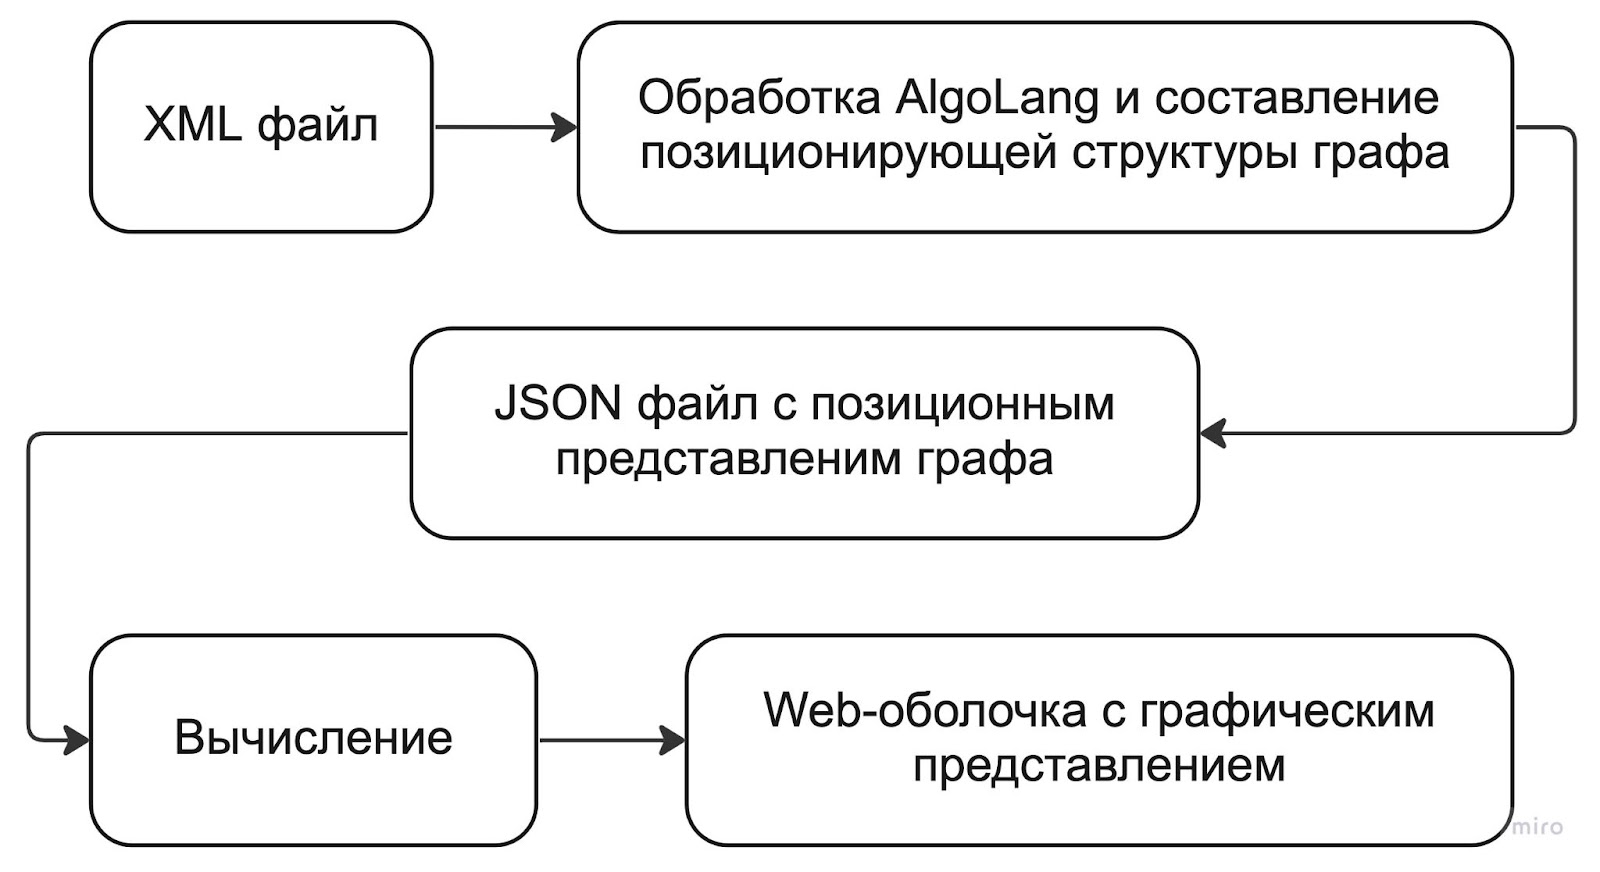
\includegraphics[width=0.9\textwidth]{assets/connection_1.jpg}
    \caption{Блок-схема способа связи двух частей системы.}
    \label{fig:connection}
\end{figure}

% As you can see in the figure \ref{fig:mesh1}, the function grows near 0. Also, in the page \pageref{fig:mesh1} is the same example.

\subsubsection{Этапы работы системы}

Работа приложения состоит из множества шагов, которые автоматически протекают на веб сервере. рассмотрим последовательность действий, начиная с загрузки пользователем файла с входными данными до получения интерактивной визуализации:

\begin{itemize}
    \item Пользователь загружает на веб страницу файл с XML структурой.
    \item Веб сервер загружает файл и запускает программу преобразования XML файла в JSON структуру.
    \item Веб сервер преобразовывает JSON структуру в файл, требуемый для его чтения программой визуализации.
    \item Веб сервер посылает ответ пользователю с новой страницей и приложением интерактивной визуализации.
    \item После загрузки новой страницы и файла, содержащего информацию о структуре графа, система создает внутреннюю структуру данных для обработки и создания 3D представления графа в виде множества 3D объектов, соответствующих и визуально описывающих все структурные элементы графа.
    \item Последним этапом является построение интерактивной визуализации полученного набора 3D-моделей, образуя вместе с пользовательских интерфейсом многофункциональную систему анализа.
\end{itemize}

\subsubsection{Docker}

Docker — программное обеспечение для автоматизации развёртывания и управления приложениями в средах с поддержкой контейнеризации, контейнеризатор приложений \cite{docker_offc}. Позволяет упаковать приложение со всем его окружением и зависимостями в контейнер, который может быть развернут на любой Linux системе.

Для быстрого развертывания приложения на удаленных серверах, вне зависимости от их конфигурации был разработан метод преобразования всего приложения в Docker образ, который способен собраться по установленным инструкциям без помощи программиста. Является важной составляющей проекта, так как приложения планируется устанавливать на нескольких серверах факультета для ознакомления и проведения учебных практикумов. Также, при помощи данного Docker образа описываемое программное обеспечение может собрать любой желающий внести вклад в развитие проекта.

\subsection{Реализованные алгоритмы оптимизации}

Возможной проблемой при реализации 3D визуализации может стать недостаток ресурсов для рендеринга сцены. Проблема решается разумным уменьшением максимально возможного числа кадров в секунду или уменьшением количества полигонов в объектах графа \cite{FastMultiDimensionalAlgorithmforDrawingLargeGraphs} \cite{Anewmethodtooptimizefor3Dlargegraphdrawing}. Однако, только этим не всегда получается оптимизировать систему до приемлемых показателей требуемой мощности вычислительных ресурсов. В рассматриваемой системе для оптимизации были реализованы несколько дополнительных методов упрощения отображения элементов.
Оптимизация моделей дуг.

Требуется использовать дуги с небольшой толщиной, однако рендеринг таких 3D моделей для этого слишком трудоемкая задача. Был адаптирован алгоритм MeshLine преобразовывающий последовательность координат в структуру простейших треугольных полигонов, представляющих собой полосу \cite{MeshLine_github}. Используя каноническое уравнение кривой программа создает 2D объект дуги, что сокращает нагрузку на графическое ядро более чем в 2 раза. Такая оценка получена эмпирическим путем сравнения результатов нагрузки на графическое ядро браузера.

\begin{figure}[!ht]
    \centering
    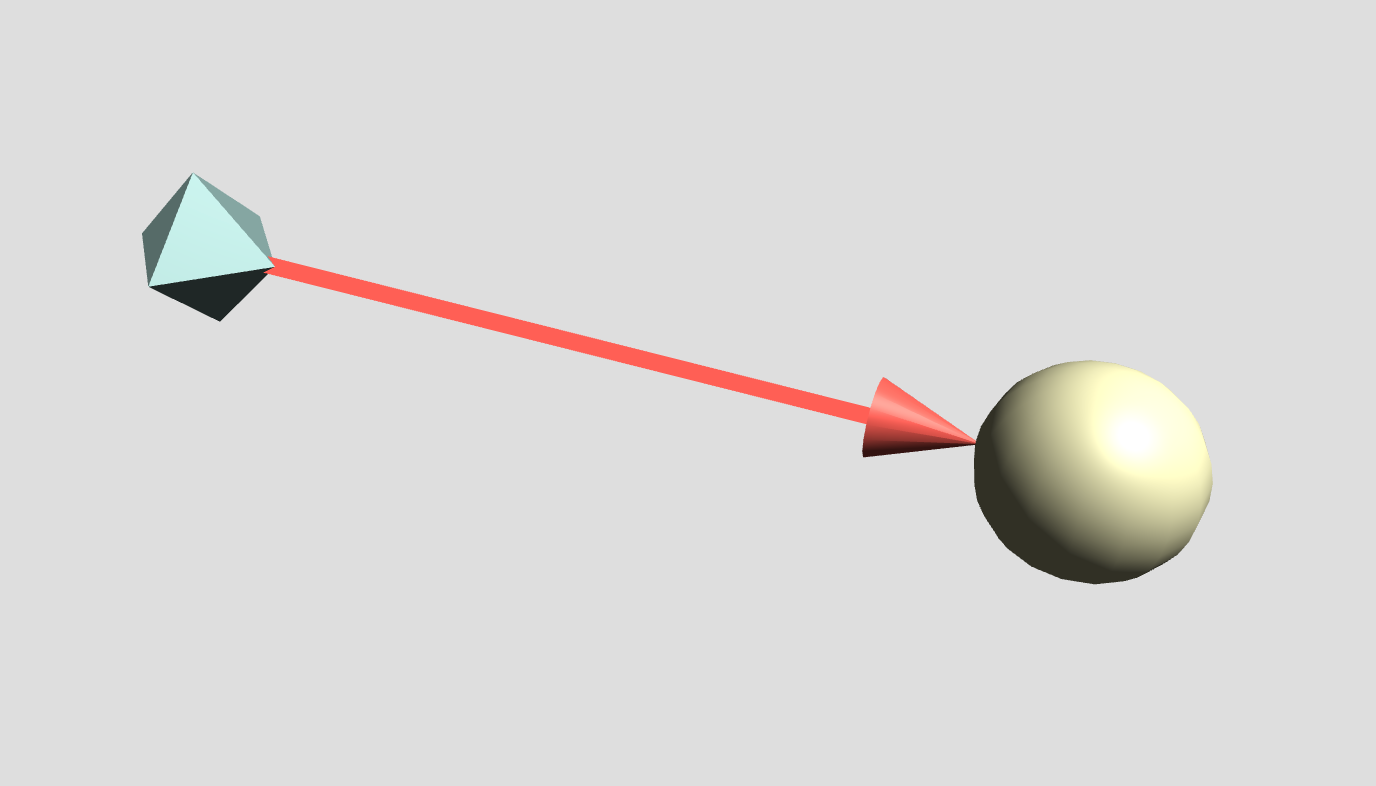
\includegraphics[width=0.6\textwidth]{assets/optimization_1.png}
    \caption{Пример 2D модели дуги в 3D визуализации.}
    \label{fig:opt_1}
\end{figure}

Оптимизация визуализации текста.
Еще один метод оптимизации, использующийся в системе – это отображение текста при помощи наложения текстур с изображением текста на невидимый спрайт, находящийся на месте требуемой подписи. Использовались алгоритмы TextSprite и TextTexture, специально разработанные для библиотеки Three.js. \cite{TextSprite_github} \cite{TextTexture_github}

\begin{figure}[!ht]
    \centering
    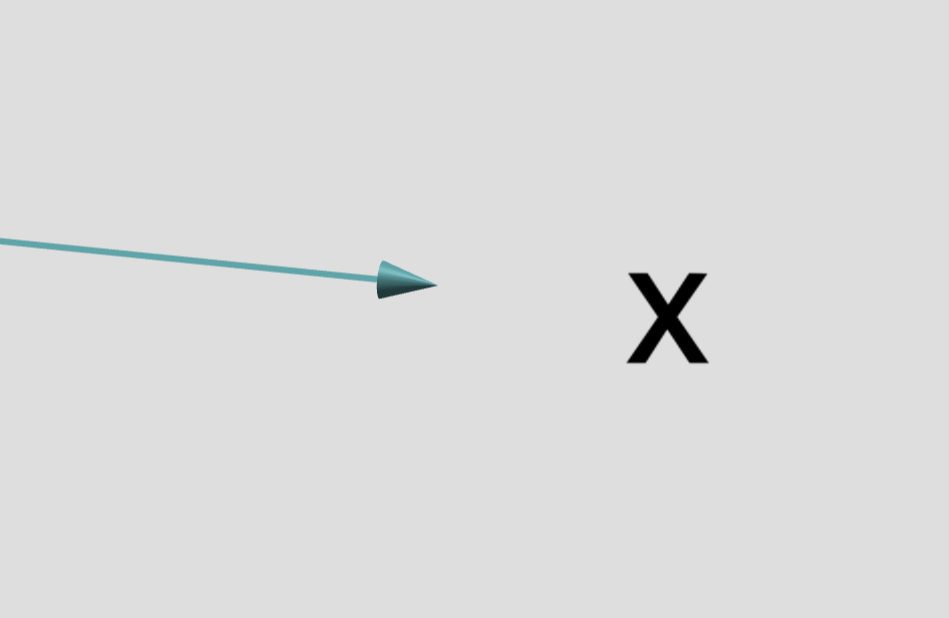
\includegraphics[width=0.6\textwidth]{assets/optimization_2.png}
    \caption{Пример оптимизированной визуализации текста.}
    \label{fig:opt_2}
\end{figure}








\subsection{Реализованная функциональность системы}
\subsubsection{Пользовательское меню управления}

Пользователю предоставляется возможность управлять графом и параметрами отображения через меню управления приложением, разработанное при помощи модуля dat.GUI. В меню есть следующие разделы:

\begin{itemize}
    \item View Settings — параметры отображения. Содержит в себе настройку ограничения FPS, ширину линий и возможность отобразить показатели нагрузки на систему.
    \item Camera Controls — настройки камеры и проекций. В этом разделе можно выбрать какой вид камеры использовать: ортогональный или перспективу. Также раздел содержит команды показа проекций графа на плоскости XY, XZ и YZ.
    \item Scene Controls — дополнительные специальные настройки.
\end{itemize}

% Внешний вид приложения показан на рисунке \ref{fig:screenshot_1}.

\begin{figure}[!ht]
    \centering
    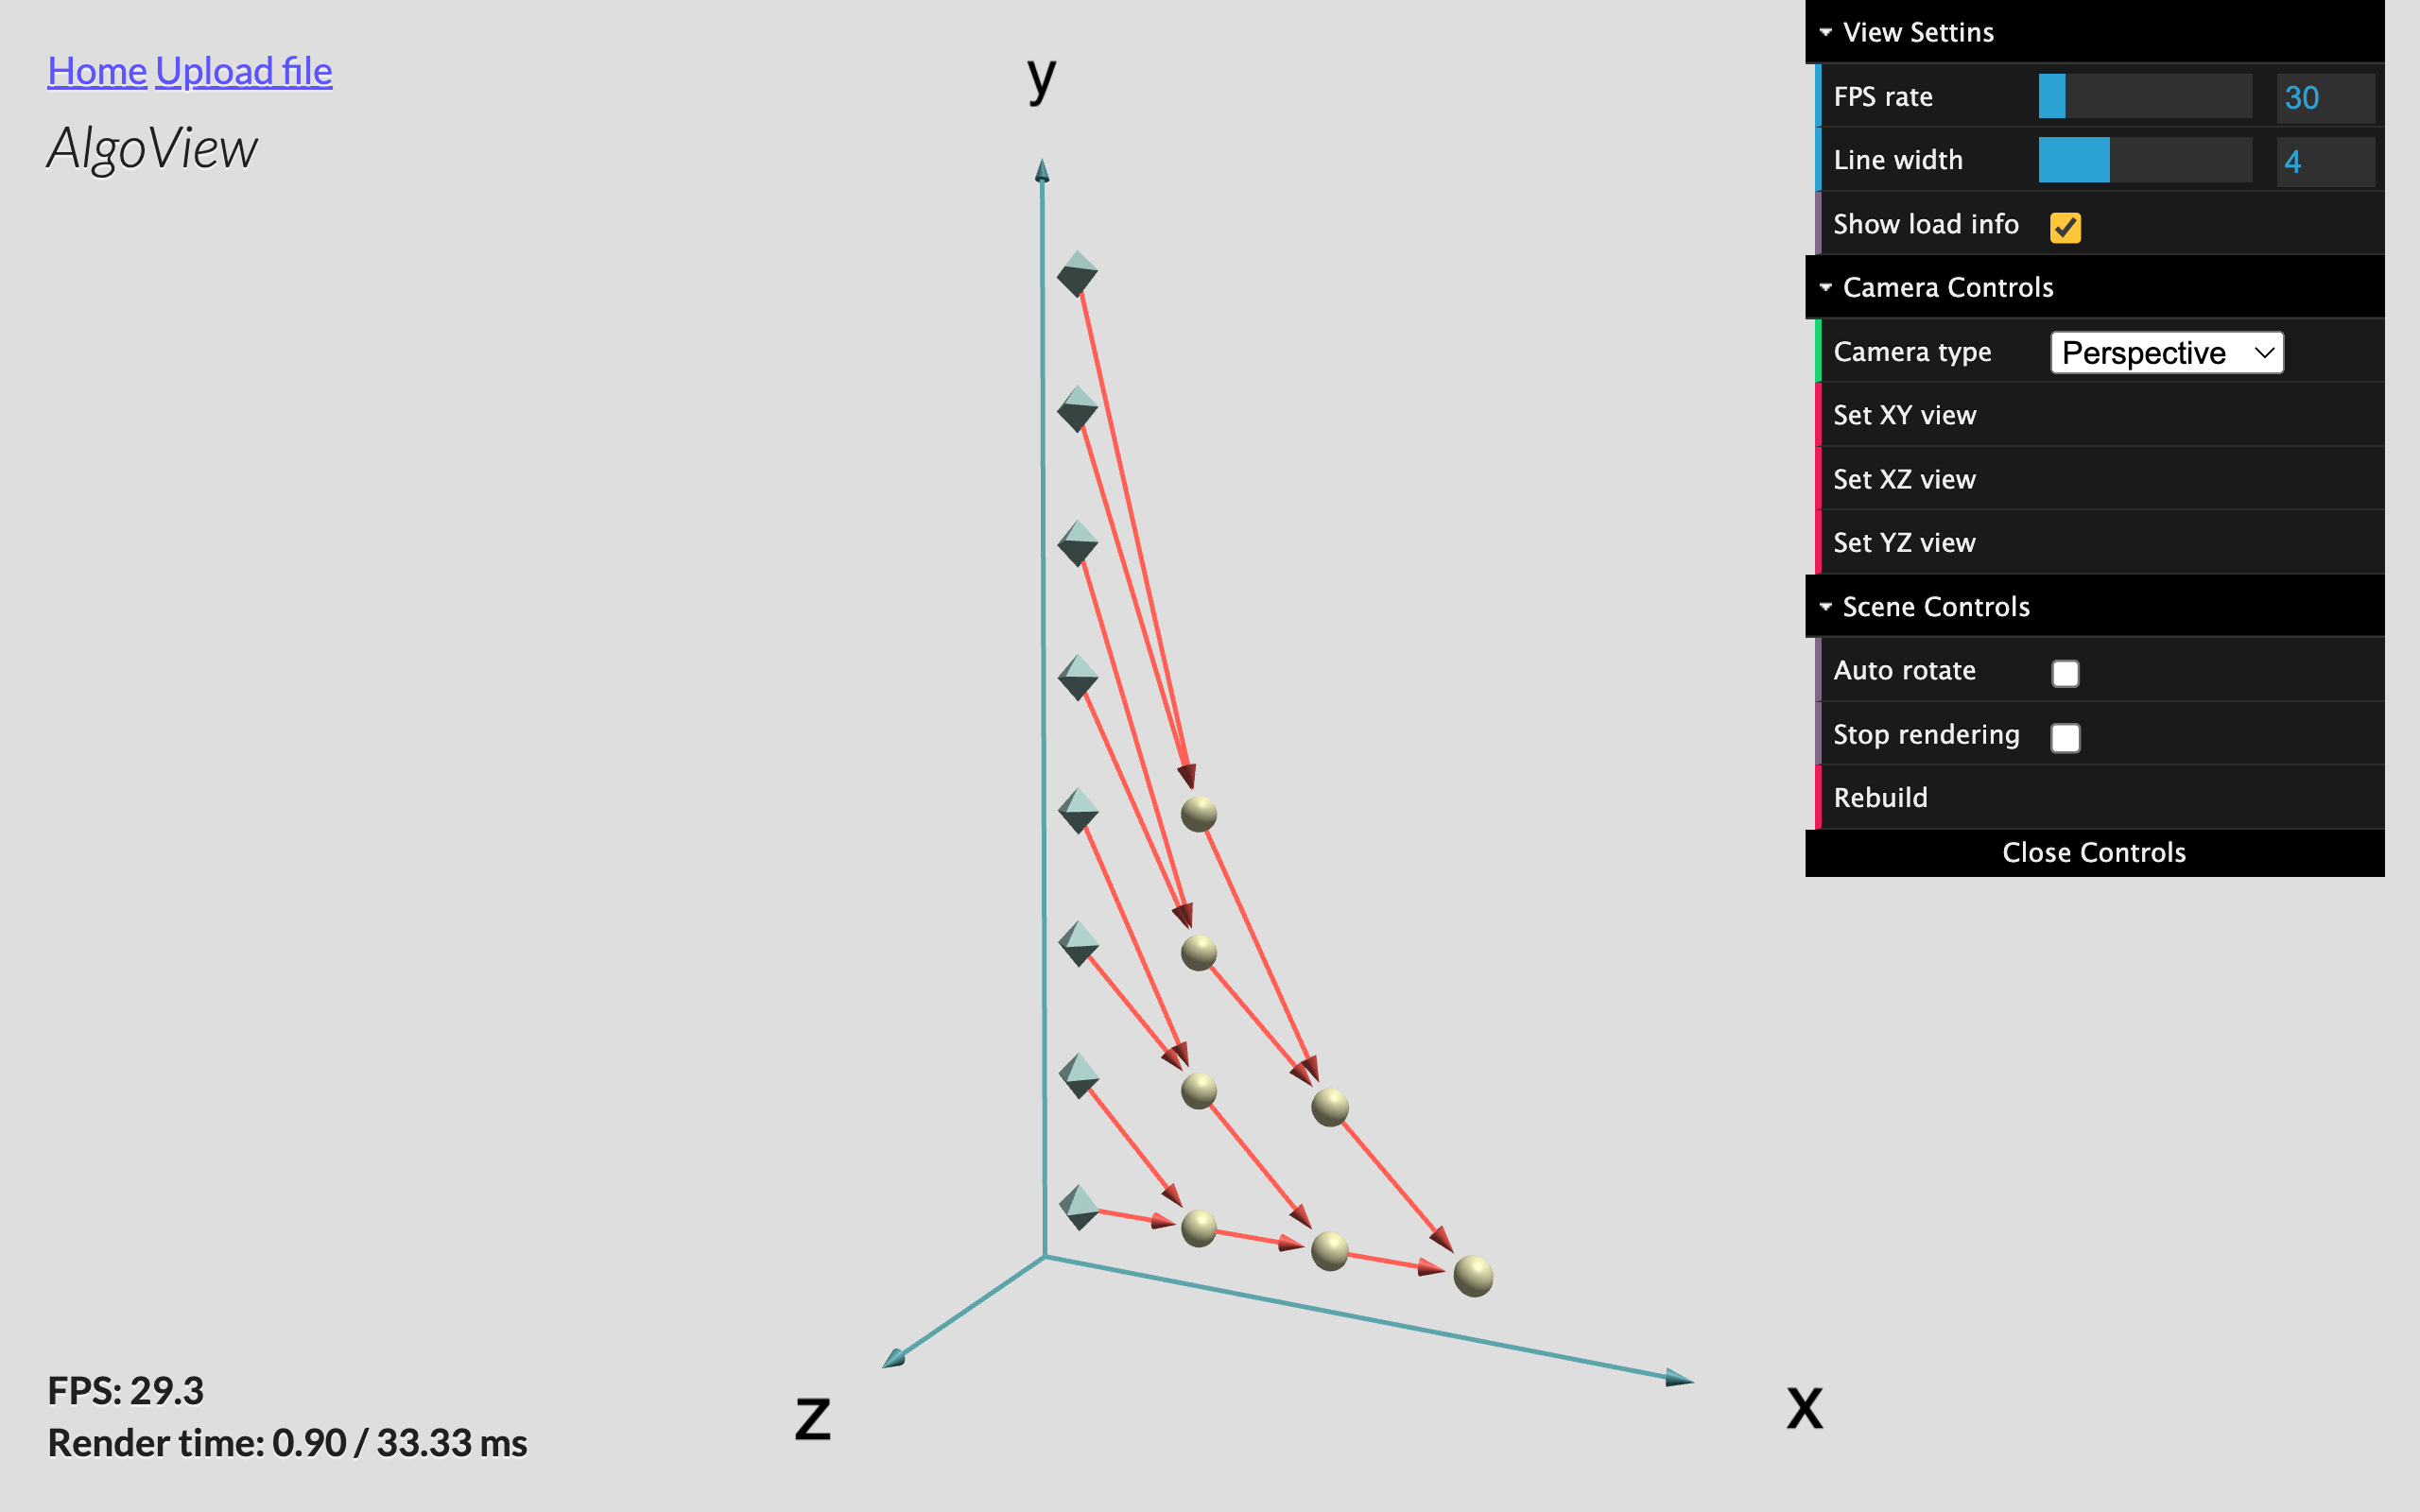
\includegraphics[width=0.95\textwidth]{assets/screenshot_1.png}
    \caption{Внешний вид приложения. Пример web 3D-визуализации (алгоритм нахождения суммы элементов массива сдваиванием).}
    \label{fig:screenshot_1}
\end{figure}

\subsubsection{Настройка камеры}

Через пользовательское меню управления в разделе Camera Controls можно выбрать какой вид камеры использовать. Ортогональный вид представляет собой изображение графа, при котором этом все компоненты имеют одинаковые размеры, независимо от положения камеры. Перспектива — изображение графа в соответствии со зрительным восприятием объектов человеком. Ортогональная камера создается встроенным конструктором THREE.PerspectiveCamera(), а с перспективой - при помощи конструктора THREE.OrthographicCamera().

\subsubsection{Проекции}

Кроме настройки камеры в разделе Camera Controls можно задать отображение проекций графа на плоскости XY, XZ и YZ. Достигается посредством позиционирования камеры в направлении желаемой плоскости.

\begin{figure}[!ht]
    \centering
    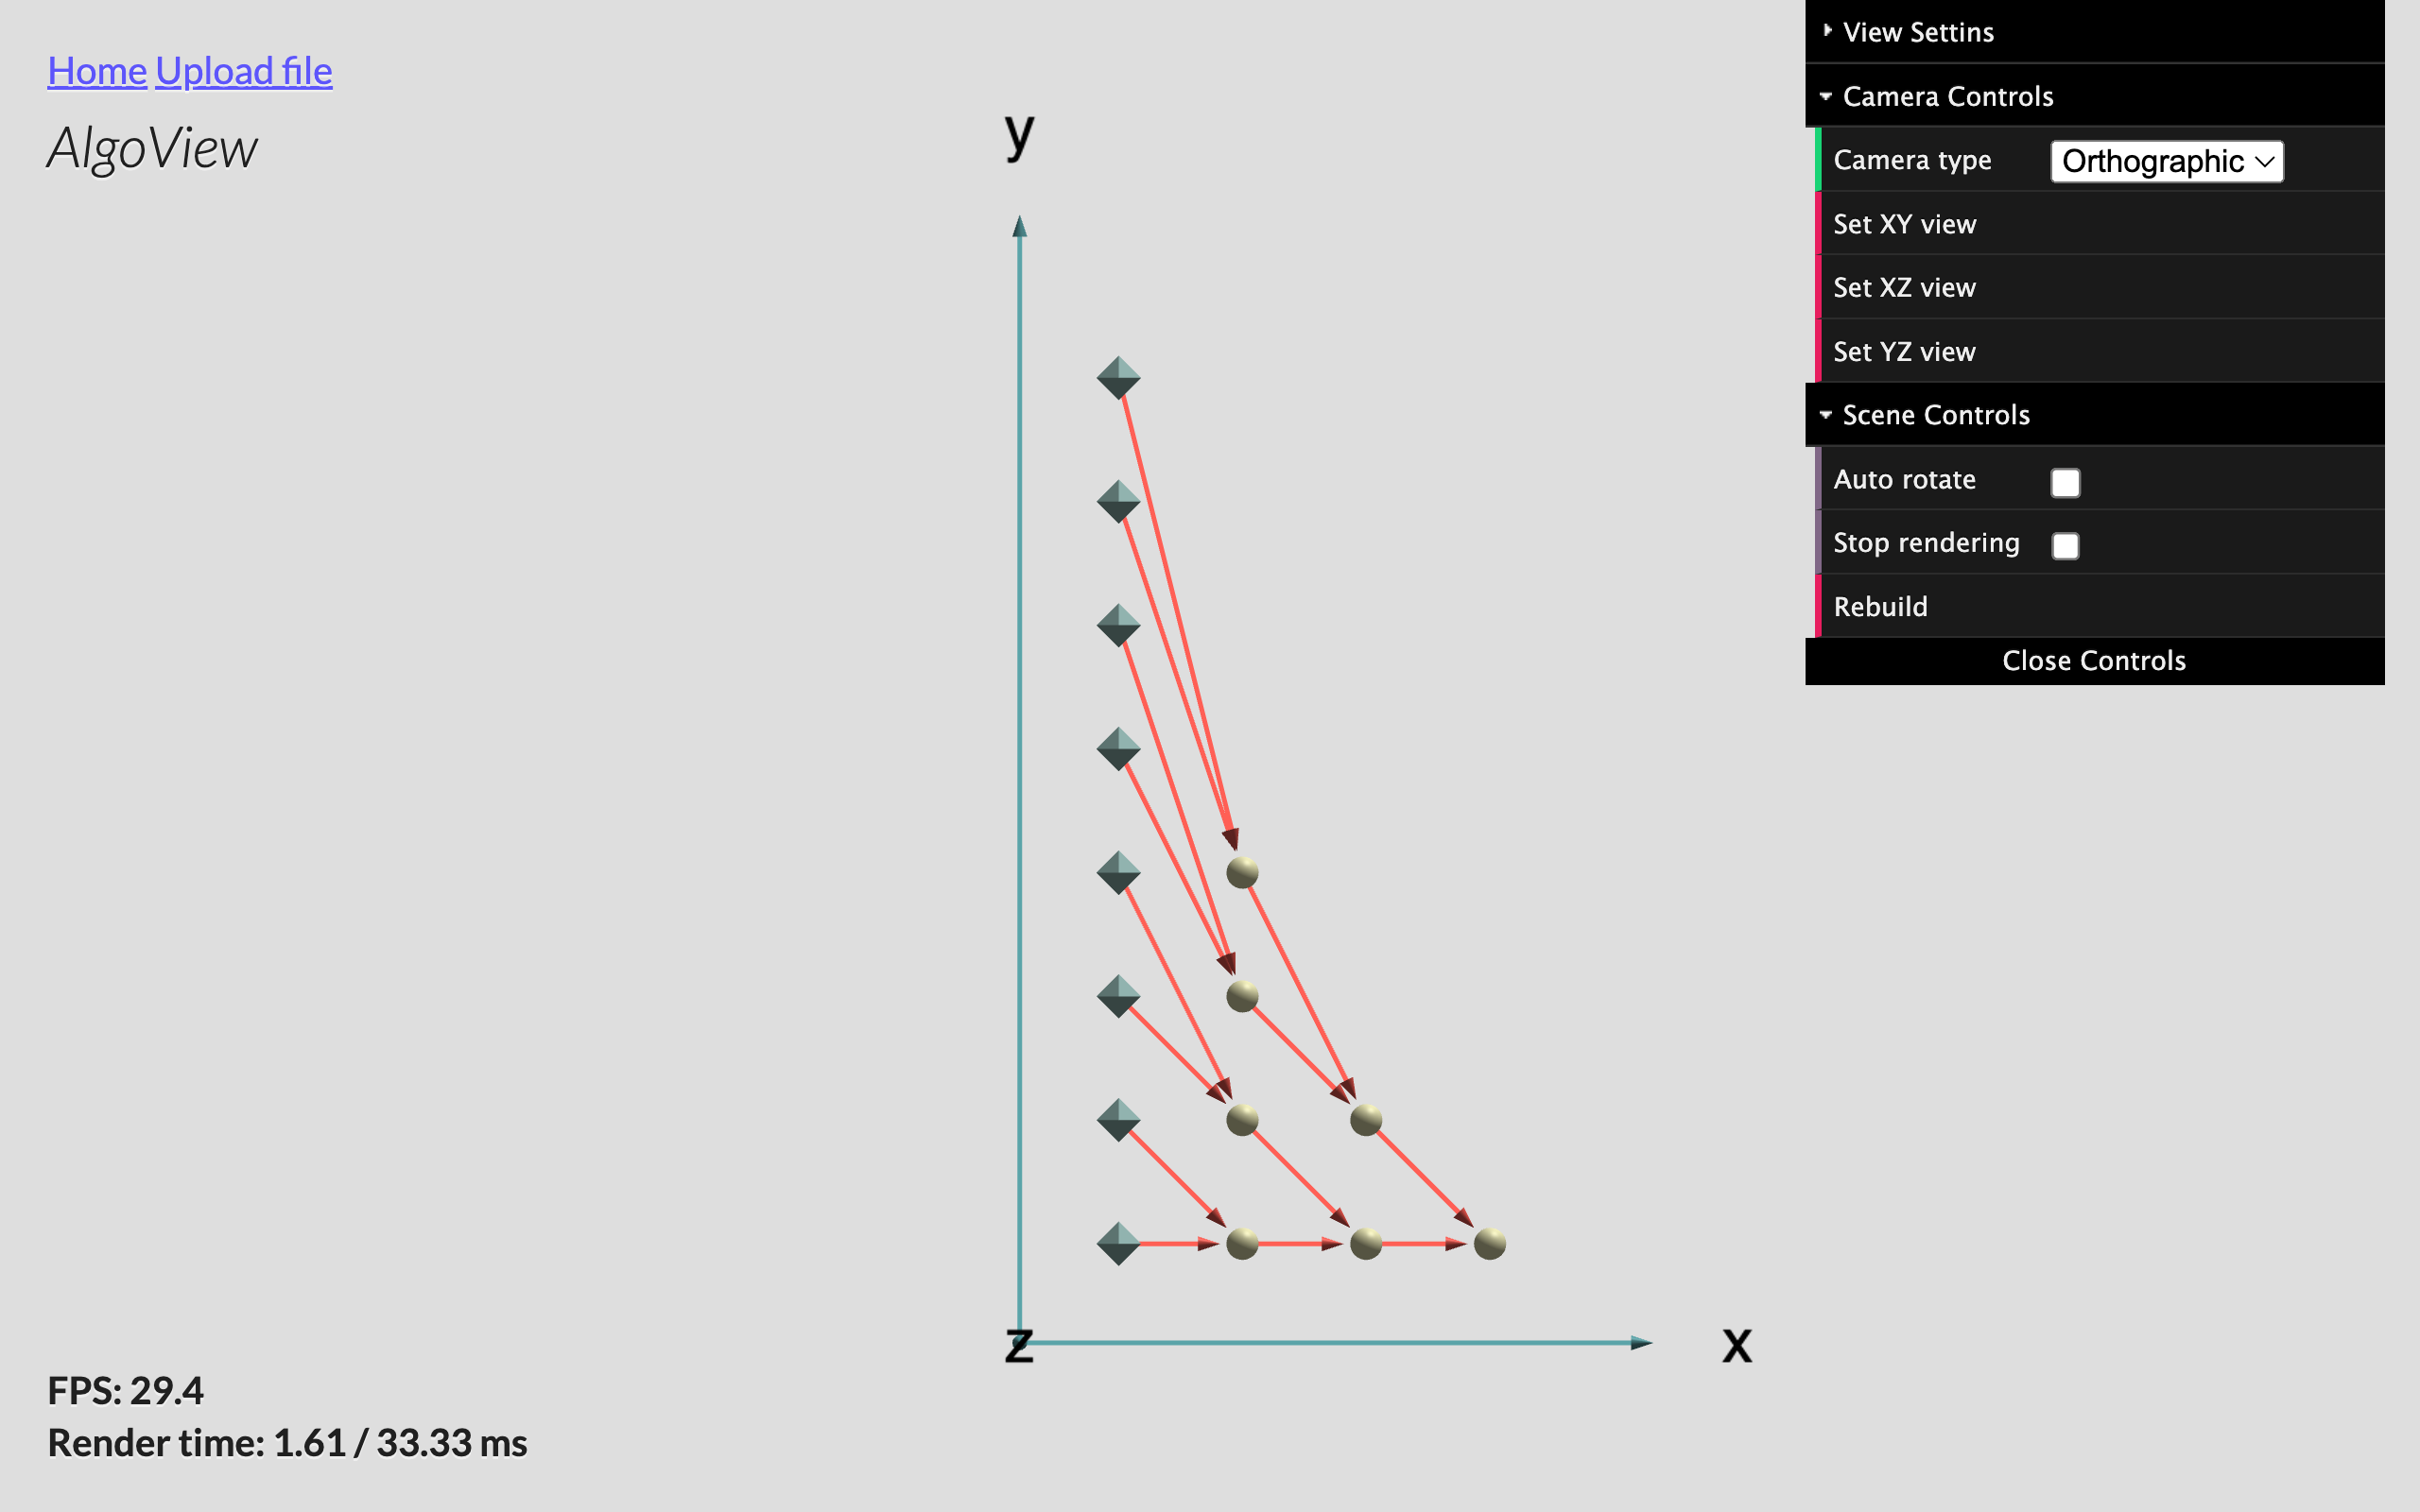
\includegraphics[width=0.95\textwidth]{assets/screenshot_2.png}
    \caption{Пример проекции на плоскость XY (алгоритм нахождения суммы элементов массива сдваиванием).}
    \label{fig:screenshot_2}
\end{figure}

\subsubsection{Управление компьютерной мышкой и клавиатурой}

Контроль над сценой реализован при помощи модуля OrbitControls в библиотеке Three. js. Удерживая левую кнопку мыши можно вращать граф. Колесиком мыши можно приближать или отдалять изображение графа. 

\subsubsection{Показатели нагрузку на систему}

Через пользовательское меню управления можно отобразить нагрузку на вычислительные ресурсы компьютера.

\subsubsection{Страница загрузки файлов}

На странице загрузки файлов  можно загрузить файл в XML формате, после чего веб сервер начнет работу по преобразованию, описанную в параграфе об этапах работы системы. Внешний вид страницы показан на рисунке \ref{fig:screenshot_3}.

\begin{figure}[!ht]
    \centering
    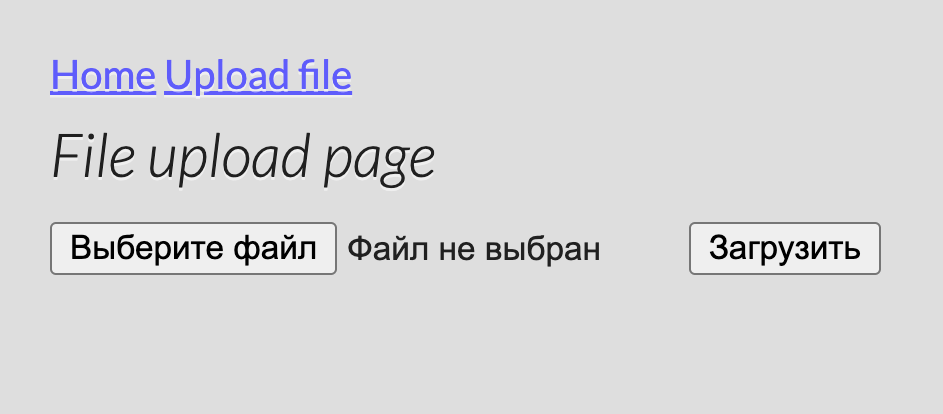
\includegraphics[width=0.95\textwidth]{assets/screenshot_3.png}
    \caption{Внешний вид страницы загрузки файлов.}
    \label{fig:screenshot_3}
\end{figure}
